
\tikzstyle{point}=[circle, draw, fill=black!50,
                        inner sep=0pt, minimum width=4pt]
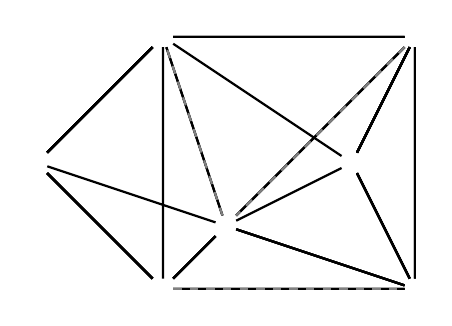
\begin{tikzpicture}[thick,scale=0.8]
 % \draw[very thin,color=gray!50] (0,0) grid (16,9);
  \draw node (a) at (1,2) {};
  \draw node (b) at (3,0) {};
  \draw node (c) at (4,1) {};
  \draw node (d) at (7,0) {};
  \draw node (e) at (6,2) {}; 
  \draw node (f) at (7,4) {}; 
  \draw node (g) at (3,4) {};
  \onslide<1>{\draw (a) -- (g) -- (b) -- (d) -- (e) -- (f) -- (c) --
    (a);}
  \onslide<2>{\draw[] (a) -- (b) -- (d) -- (e) -- (f) -- (c)
    -- (g) -- (a);
  }
  \onslide<3>{\draw[] (a) -- (b) -- (d) -- (f) -- (e) -- (c)
    -- (g) -- (a);
  }
  \onslide<4>{\draw[] (a) -- (b) -- (c) -- (d) -- (f) -- (e) -- (g) -- (a);
  }
  \onslide<5>{\draw[] (a) -- (b) -- (c) -- (d) -- (e) -- (f) -- (g) -- (a);
  }
  \onslide<6>{
    \draw[] (a) -- (b) -- (c) -- (d) -- (e) -- (f) -- (g) -- (a);
  }
 \onslide<7>{
    \draw[] (a) -- (b) -- (c) -- (d) -- (e) -- (f) -- (g) -- (a);
    \draw[color=gray,dashed] (b) -- (d);
    \draw[color=gray,dashed] (f) -- (c);
    \draw[color=gray,dashed] (c) -- (g);
 }

\end{tikzpicture}
